
RQ1 gets answered here, working through the protocol (\S{}4.1), headline recall (\S{}4.2), audited precision (\S{}4.3--\S{}4.4), the hardest predicate pair broken down per annotator (\S{}4.5), the residual human cost (\S{}4.7), every remaining miss diagnosed (\S{}4.10), and full automation with a detector in the loop (\S{}4.11). Each measure is bounded by the labels it is scored against, so \S{}4.12 and \S{}4.13 drop the gold and ask two other questions: whether the labels survive the camera moving, and whether a vision-language model would have done the job. Three further studies use no gold and sit in Supplementary E, covering out-of-domain video (E.3) and 1,766 unlabelled robot frames (E.5).

\section{Protocol}

Four counts come up repeatedly below. Of the released subset, \textbf{884} frames are present. \textbf{838} carry a non-empty annotation. The pipeline runs on \textbf{836}, because two annotation files have no matching image (\S{}4.2). And \textbf{802} of those give at least one ordered pair, the other 34 holding a single object. Two properties of the gold end up shaping the whole protocol. It is \textbf{sparse}, since only 8,790 of 84,880 ordered pairs (\textasciitilde{}10\%) carry a human label, so a label missing from the gold is unexamined rather than wrong, and raw precision undercounts. Those 8,790 pairs hold 8,926 triplets, 136 of which carry a second predicate, which is why the pair and triplet counts never match. Annotator behaviour is also \textbf{uneven} (Chapter 3 for \texttt{near}, \S{}4.5 for a second case), so agreement is reported per annotator group as well as pooled.

For measurements I use per-predicate \textbf{recall of the human triplets}, which is the primary one and follows the source paper's convention; \textbf{restricted precision, recall and F1} on annotated pairs; a \textbf{manual audit} of a stratified sample of the extra predictions; per-type \textbf{flag rates}; and three baselines, random, majority and \textbf{box-only geometry}. Boxes and classes are ground truth throughout (PredCls), so box IoU does not apply. Thresholds were fitted on annotator groups 0--5 only, with 6--8 held out. Each group is also a contiguous block of the capture, so the split holds out an unseen arrangement as well as an unseen annotator (\S{}4.12). Figure~\ref{fig:qualitative-examples} shows what the tool emits on two frames, one from a calibration group and one held out.
\begin{figure}[!htbp]
\centering
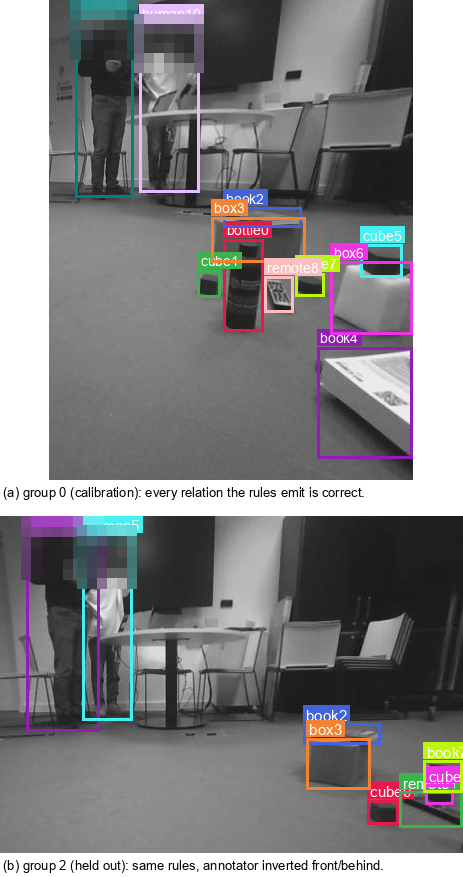
\includegraphics[width=0.80\textwidth,height=0.78\textheight,keepaspectratio]{figures/qualitative-examples.png}
\caption[Two scenes as the pipeline labels them, with the detected]{Two scenes as the pipeline labels them, with the detected boxes and class instances drawn. Left, a calibration group on which every emitted relation is correct. Right, a held-out group whose annotators recorded front and behind under the opposite convention, which is the failure Section 4.5 decomposes. Faces are pixelated from the dataset's own human boxes, as Section 3.12 requires of anything republished.}
\label{fig:qualitative-examples}
\end{figure}


\section{Headline: recall of the human triplets}

Figure~\ref{fig:rq1-recall} plots the per-predicate result. Baselines are added in the table.
\begin{figure}[!htbp]
\centering
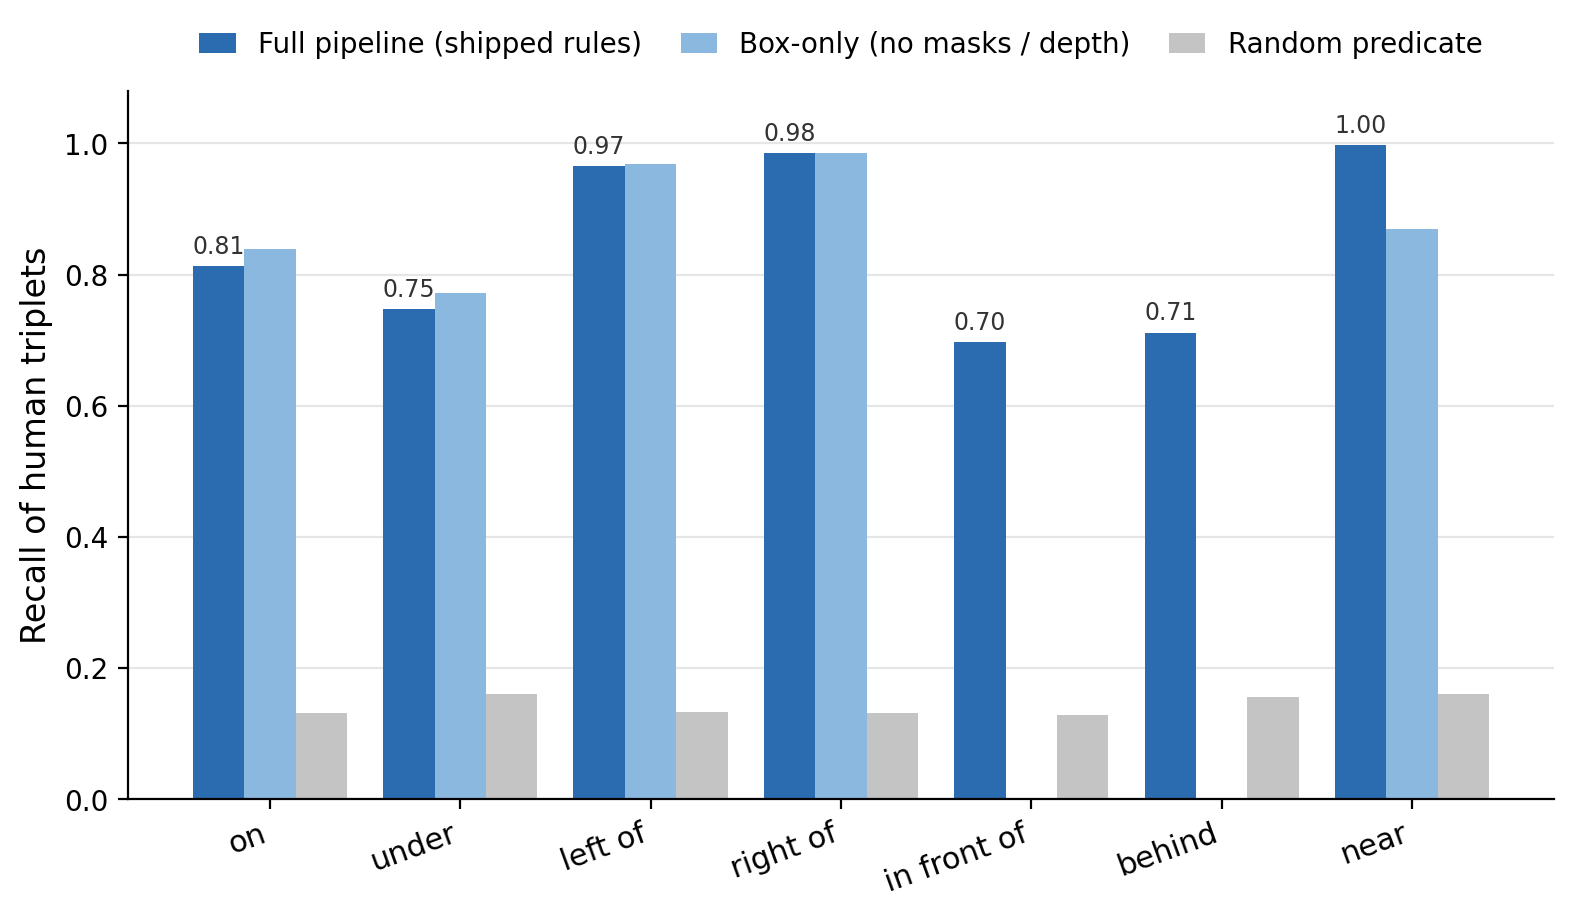
\includegraphics[width=0.80\textwidth,height=0.78\textheight,keepaspectratio]{figures/rq1-recall.png}
\caption[Recall of the human triplets per predicate]{Recall of the human triplets per predicate: the full pipeline against a box-only ablation and a random baseline. Front and behind have no box-only bar because that ablation cannot compute depth.}
\label{fig:rq1-recall}
\end{figure}


\needspace{15.8\baselineskip}
\begin{center}
\setlength{\tabcolsep}{6pt}
\small
\begin{longtable}{lrrlrrr}
\caption[Per-predicate recall of the human triplets, pooled]{Per-predicate recall of the human triplets, pooled and on held-out annotators, against three baselines. *the majority baseline emits ``in front of'' everywhere, trivially recalling that class and nothing else; \textdagger{}near rounds 715/717 = 0.997 (\S{}4.9), on a predicate whose precision on annotated pairs is 0.11, not comparably high (\S{}4.3).}\\
\hline
Predicate & Gold & Ours & \textbf{Ours (held-out)} & Random & Majority & Box-only \\
\hline
\endfirsthead
\hline
Predicate & Gold & Ours & \textbf{Ours (held-out)} & Random & Majority & Box-only \\
\hline
\endhead
on & 1465 & 0.81 & \textbf{0.85} & 0.13 & 0.00 & 0.84 \\
under & 1001 & 0.75 & \textbf{0.82} & 0.16 & 0.00 & 0.77 \\
to the left of & 972 & 0.97 & \textbf{0.95} & 0.13 & 0.00 & 0.97 \\
to the right of & 1174 & 0.98 & \textbf{0.99} & 0.13 & 0.00 & 0.99 \\
in front of & 2013 & 0.70 & \textbf{0.20} & 0.13 & 1.00* & 0.00 \\
behind & 1584 & 0.71 & \textbf{0.37} & 0.16 & 0.00 & 0.00 \\
near & 717 & 1.00\textdagger{} & \textbf{1.00} & 0.16 & 0.00 & 0.87 \\
\textbf{mean} & 8,926 & \textbf{0.85} & \textbf{0.74} & 0.14 & 0.14 & 0.63 \\
\hline
\end{longtable}
\end{center}

The held-out front/behind cells (0.20/0.37) are dominated by two held-out groups that labelled the pair under the \textit{opposite direction convention}. Section 4.5 takes that apart, and convention-aligned depth recall is 0.91 pooled. Because every human triplet is scored, these are population values. Whether another batch would agree is a different question, answered by a cluster bootstrap over images (\texttt{eval/uncertainty.py}), where the widths, not the centres, carry the argument, and the held-out intervals appear in \S{}4.6. Those intervals are nominal, not calibrated. Section 4.12 establishes that the images are consecutive frames of one trajectory, so resampling them as independent draws understates the true width (Supplementary F.8). Three readings sit underneath the table, given in Supplementary F.11. The tool recovers \textbf{81\% of all human triplets} (7,276 of 8,926) against 14\% for random and 23\% for majority on the same triplet-weighted basis. Box-only geometry matches it on the laterals but not on support quality or \texttt{near}, and cannot compute the depth pair. And held-out beats pooled on on/under/near while collapsing on front/behind. Both are annotator signatures, and neither is a property of the geometry. Gold totals 8,926, not 8,928, because two stray annotation files without matching images are excluded.

\section{Precision on the annotated pairs}

Restricted to the 8,790 annotated pairs, precision runs 0.95 and 0.92 on the support pair, 0.35 and 0.42 on the laterals, 0.43 and 0.35 on the depth pair and 0.11 on \texttt{near} (Supplementary F.6). Every one of those is bounded below by construction. The human typically recorded one or two relations where several hold at once, and \texttt{near} is the extreme case, emitted wherever the fitted gap holds while three of nine groups supplied all but three of its labels. That is why the protocol includes the audit (\S{}4.4), and why I do not read these columns at face value.

\section{Manual audit of extra predictions (audited precision)}

105 extra predictions (15 per predicate, seeded stratified sample) were rendered with subject/object boxes and verdicted by hand, any case not clearly true marked wrong (\texttt{outputs/audit/audit\_\allowbreak{}sheet.csv}), and since that audit ran against the \textit{pre-gate box rule} I report it as found, because it motivated the support-rule repairs. Section 4.14 traces the whole arc, running 0.13 to 0.77 unblinded, then 0.40 blind against decoys, then 0.54 after the refit. So the support figures here describe a failure I later fixed, not the final tool. That audit splits the predicates in two. For lateral, depth and proximity, \textbf{every sampled extra prediction was correct} (15/15 each, Wilson 95\% [0.80, 1.00]), so \S{}4.3's low restricted precision is the sparse-gold artefact the protocol anticipated. For support it inverts. \texttt{on} scores 1/15 (0.07, [0.01, 0.30]) and \texttt{under} 3/15 (0.20, [0.07, 0.45]), mostly \textbf{false fires} of box adjacency on objects that merely project next to each other. Together with \S{}4.2's containment misses, both error directions point at one repair, a mask-contact test, which the ablations evaluate. Two caveats are worth stating. 15 per predicate gives wide intervals, and depth verdicts on near-coincident objects were occasionally marginal.

\section{The front/behind decomposition: a second measured annotation defect}

Figure~\ref{fig:front-behind-decomposition} breaks front/behind down by annotator group, with the two convention-inverted groups sitting alone near zero, and Supplementary F.10 carries the per-group table. Pooled at 0.70, the figure resolves into three causes in measured proportions. \textbf{Direction agreement is near-perfect where the tool commits}, 0.95--1.00 for six of the eight groups with meaningful counts, so genuine depth-ordering errors are rare. \textbf{Two annotator groups used the inverted convention}, agreeing 2--5\% of the time, so flipping their labels recovers 0.94/0.82 and aligned overall recall is 0.91. And \textbf{the remaining gap is abstention, not error}, with groups 2 and 3 agreeing almost perfectly when the tool commits, but sitting inside the \texttt{depth\_\allowbreak{}eps} band and beyond the fallback's reach. After \texttt{near}, this is the second measured annotation defect, the reference-frame ambiguity RoboSpatial formalises (\S{}2.5), observed in the wild. What rules out simple subjectivity is the shape of the distribution. A contested judgement would scatter agreement around chance. These two groups sit at 0.02--0.05 and the other six at 0.95--1.00, and agreement that far \textit{below} chance is a sign flip, not a difference of opinion. Neither convention is the wrong one.
\begin{figure}[!htbp]
\centering
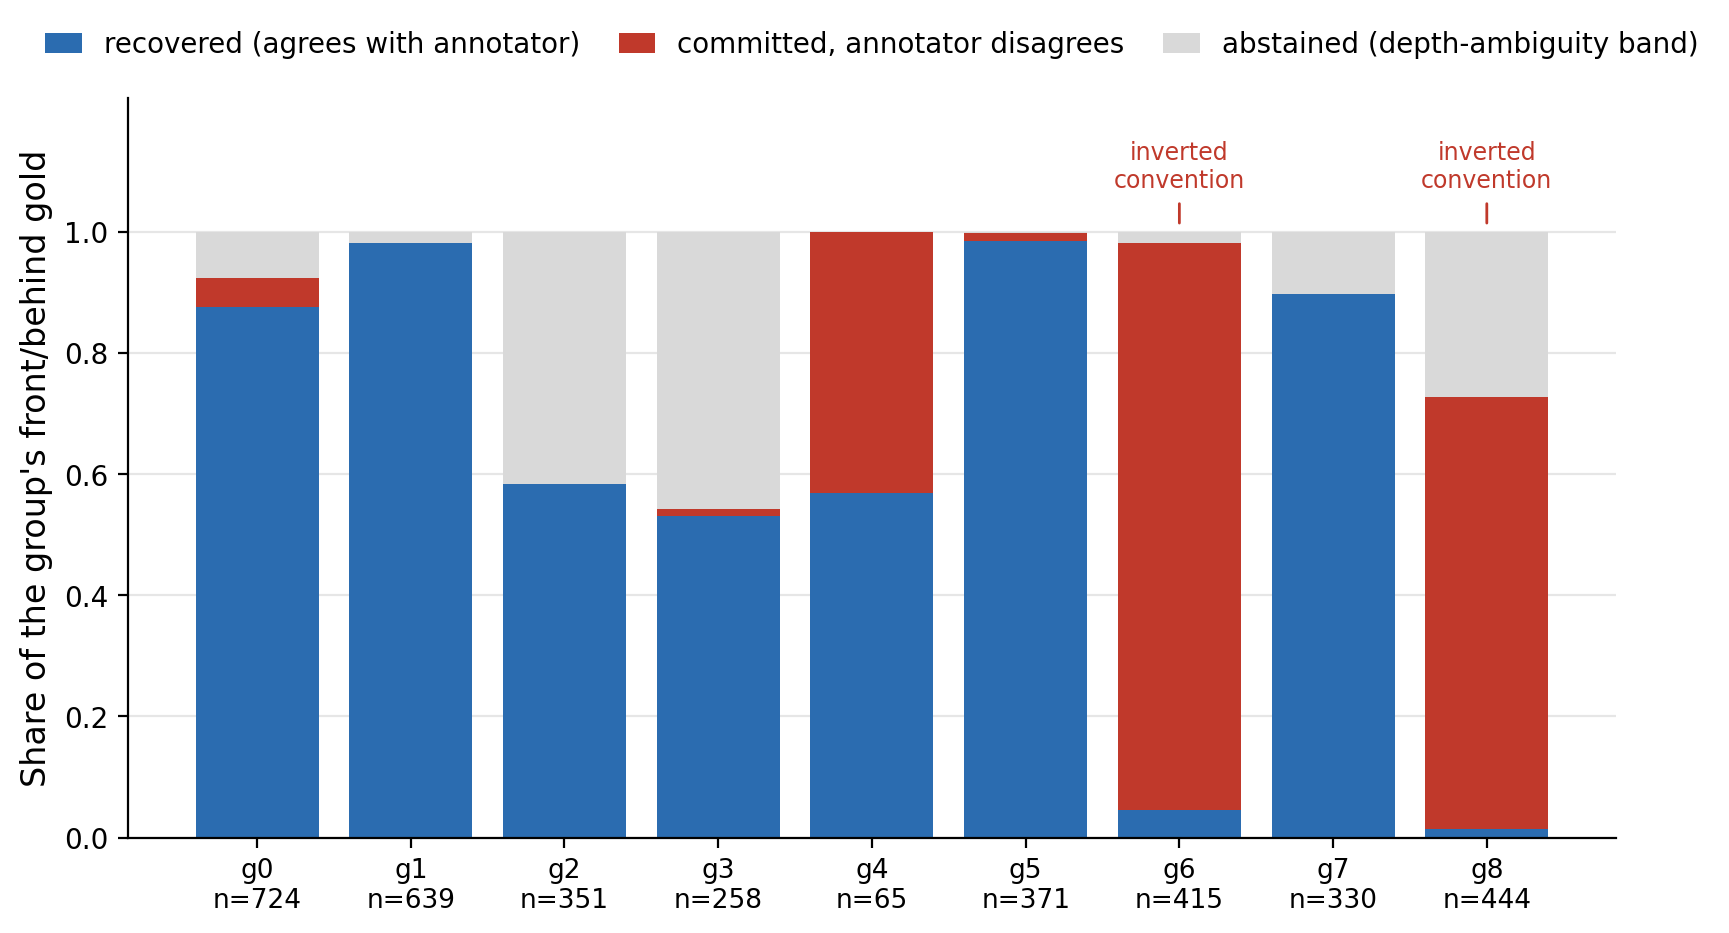
\includegraphics[width=0.80\textwidth,height=0.78\textheight,keepaspectratio]{figures/front-behind-decomposition.png}
\caption[Front/behind decomposed per annotator group]{Front/behind decomposed per annotator group: agreement where the tool commits, deliberate abstention, and the two groups that used the inverted direction convention.}
\label{fig:front-behind-decomposition}
\end{figure}


\section{The tenth annotator, and what the annotators would score against each other}

Per-group recall of each annotator's triplets, all predicates: group\_\allowbreak{}0 0.85 $\cdot$ group\_\allowbreak{}1 0.90 $\cdot$ group\_\allowbreak{}2 0.92 $\cdot$ group\_\allowbreak{}3 0.88 $\cdot$ group\_\allowbreak{}4 0.86 $\cdot$ group\_\allowbreak{}5 0.93 $\cdot$ group\_\allowbreak{}6 0.56 $\cdot$ group\_\allowbreak{}7 0.90 $\cdot$ group\_\allowbreak{}8 0.57. Almost all of that spread comes from the two convention-inverted groups. The tool agrees with the \textit{consistent} annotators at 0.85--0.93, a band the support refit of \S{}4.14 tightened by lifting group 3 from 0.72. On the held-out annotators the cluster-bootstrap intervals of \S{}4.2 put five of the seven predicates at 0.82 or better, with the depth pair far below at 0.199 (0.148--0.257) and 0.369 (0.300--0.443), a gap much wider than the sampling uncertainty. That is what makes \S{}4.5's convention explanation a claim about the labels, not about noise (all seven intervals in Supplementary F.8). A quality verdict needs a measure the dataset does not supply, how well two \textit{human} annotators would agree, and because the groups labelled disjoint batches it cannot be measured directly, which is itself a finding about how the dataset was built. Treating the deterministic tool as a fixed common reference (\texttt{eval/annotator\_\allowbreak{}agreement.py}) does bound it. Across the seven consistent groups its agreement spans \textbf{0.851 to 0.933} about a mean of 0.892. That is an \textbf{upper bound on annotator heterogeneity, not a measurement of it}, because the nine batches differ threefold in object density, so the spread carries batch difficulty as well as annotator behaviour. The same non-exchangeability defeats the Fréchet route to a tighter bound. Supplementary F.7 gives the derivation, the interval it produces, the density figures, and why the assumption behind it is false here, not merely unverified. No inter-annotator agreement figure can be got out of this dataset, even by bounding. A replication that wants one has to collect overlapping assignments. So RQ1's comparability claim rests on the trivial baselines and the per-predicate audit (\S{}4.8).

\section{Flags: what review actually costs}

31.5\% of ordered pairs carry at least one flag. Those kinds overlap, so they sum past that (Supplementary C.9). Depth-ambiguous is 19.3\%, down from 29.5\% before the ground-plane fallback resolved a third of the depth abstentions, and lateral-ambiguous is 10.0\%. Both are \textit{abstentions}, with nothing to review. The borderline-near band, 8.5\% of pairs, is the genuine review queue. At a conservative 3 seconds per queued pair that is roughly 6 hours for the full dataset, against the original nine-annotator manual pass, and it is optional for the fidelity reported above. What survives in the released materials is vocabulary lists, so Chapter 3's specification is the first \textit{executable} definition of these predicates, which \S{}7.3 draws out.

\section{Answer to RQ1}

The two axes divide the seven predicates differently, which I say plainly and do not fold into a single headline. On \textbf{recall}, five reach human-comparable levels, 0.75 to 1.00 in Table 4.1, with mean 0.85 and 0.74 on annotators no threshold ever saw, the exception being the depth pair at 0.70/0.71 pooled and 0.91 once the two inverted groups are aligned. On \textbf{precision}, a different five audit blind at 0.79--1.00, the two laterals, the two depth predicates and \texttt{near}, each on 24 samples. Those are two different fives. The first is recall against annotators no threshold saw; the second is audited precision on labels no annotator wrote. What they jointly support is weaker than comparability with the human process, for the reason \S{}4.6 gives. The exception there is support, at \textbf{0.535 [0.42, 0.65]} on 71 samples of the shipped rule, up from 0.404 before \S{}4.14 traced the shortfall to a threshold fitted on a metric that could not see the error it controls. No predicate is weak on both axes, and none is strong on both except the laterals and \texttt{near}. Support recalls well but cannot be trusted where it adds. The depth pair is trustworthy where it commits, and it commits less often than the annotators did. Supplementary F.12 sets out why that structure makes a per-predicate answer necessary, and F.11 why \texttt{near}'s 0.997 most overstates what is known. Section 8.1 answers RQ1 against the criteria of \S{}1.2.2 on this basis, and the residual human cost is an 8.5\% review queue (\S{}4.7) against labels 20$\times$ denser than the human set.

\section{Shipped from the ablations}

Ten ablations were run. Seven sweep a shipped parameter over the cached geometry and re-run offline in about twenty seconds (\texttt{eval/ablations.py}). Two test whether a heavier perception stack would do better, and one tests whether geometry can replace the class guard. All three say no. Every parameter was selected on the training annotator groups alone, with the held-out column reported and never optimised against. Supplementary D.0 tabulates each ablation, its shipped setting and its verdict, with D.1--D.8 giving the derivations, and on three the headline table moved materially, in this order. My audit localised a support precision failure. A geometric insight, that stacked objects share a camera distance, fixed half of it (A1, held-out support F1 0.58 $\rightarrow$ 0.71). Mask-bottom contact fixed most of the rest while \textit{raising} recall, 0.71 $\rightarrow$ 0.87 (A5). And the ground-plane fallback recovered most of the front/behind abstention band without using depth at all, taking 0.52/0.55 $\rightarrow$ 0.70/0.71 and mean recall 0.79 $\rightarrow$ 0.85 (A7). Two declined perception ablations bound where engineering can help. Neither a four-times-larger depth model (A8) nor two-view triangulation (A9) improves the depth pair, and the second is 0.20 \textit{worse} where it answers, on 9\% of pairs. What limits it is monocular ambiguity in the scenes, not model capacity. What I decline is a lightweight uncalibrated estimator, not multi-view geometry in general, so a calibrated stereo pair stays open as the route \S{}8.3 keeps.

\section{Failure gallery: every miss diagnosed}

Every missed human triplet is diagnosed automatically, by re-checking the rule's conditions against the cached geometry and mask-contact maps (\texttt{scripts/make\_\allowbreak{}failure\_\allowbreak{}gallery.py}; rendered examples in \texttt{outputs/failure\_\allowbreak{}gallery/}). Supplementary D.7 breaks the 1,650 misses of the shipped rule set down by predicate and cause. Genuine depth-ordering errors remain 1--6\% of front/behind misses, the support misses are threshold trades on real contact evidence, and \texttt{near} misses have all but vanished. That convention-inverted \textit{share} grew to 45--51\%, not because those misses increased but because the fallback shrank the abstention share around them, with total misses falling from 2,107 to 1,650. Misses attributable to avoidable tool error across all seven predicates: \textasciitilde{}7\%.

\section{Detector-in-the-loop: full automation, attributed}

In deployment mode the ground-truth boxes are replaced with Grounding DINO (Liu et al., 2024) zero-shot detection, on the identical SAM2 $\rightarrow$ depth $\rightarrow$ rules stack (\texttt{scripts/run\_\allowbreak{}sgdet.py}). End-to-end triplet recall over 836 images is \textbf{0.38} against the PredCls headline, and the decomposition attributes most of that gap. Zero-shot detection recall spans 0.40 (cube) to 0.95 (human), a triplet needs \textit{both} endpoints, and \textbf{conditioned on both being detected the relation layer scores 0.85 mean, matching PredCls}. Detection is the dominant term, though not a complete accounting, since missed objects also change which pairs get presented, and the rules are detector-agnostic. Two caveats. Zero-shot open-vocabulary detection is the worst-case detector, the trade \S{}2.6 identifies, used here because the authors' trained YOLOv10m weights were not available. And the 20-image tuning trial over-estimated detection quality, because its scenes all came from one annotator batch. On two out-of-domain clips the same attribution holds, every visible failure again being a detection failure (Supplementary E.3).

\section{Temporal redundancy and stability under viewpoint change}

The 884 released images are one continuous walk, with each annotator group a contiguous 100-frame block, so \S{}4.1's held-out split is held out by scene as well as by annotator. The annotator reading survives that, because an inverted convention (\S{}4.5) and a \texttt{near} label used in quantity by three groups in nine are behaviours no arrangement of furniture can produce. The confound also runs favourably, since 0.74 on held-out groups is generalisation to an unseen annotator \textit{and} an unseen arrangement, and the sequence lets the verdicts be checked against themselves with no human labels, which Supplementary E.2 carries in full.

Two results. Skipping frames costs nothing measurable, with mean recall 0.832 propagated against 0.829 per frame at every threshold tested. And the stability finding is not the expected one. Front/behind, the predicted loser if its errors were depth noise near the boundary, agrees with itself \textbf{0.958} of the time, above \texttt{on}/\texttt{under} at 0.878 (mean 0.946), and still 0.911 at 89$\times$ compression. A predicate recalling 0.648 of the human labels while agreeing with itself at 0.958 is making the same call repeatedly and disagreeing systematically, which converges with A8 and \S{}4.5. Section 7.2 develops what follows from that. \textbf{Limits:} consistency is not correctness, since a systematically wrong rule is perfectly stable too, so 0.958 rules out only the depth-noise explanation this section was written to test, and the figures are an upper bound anyway, since only matched pairs contribute (E.2).

\section{Would a vision-language model do this instead?}
\begin{figure}[!htbp]
\centering
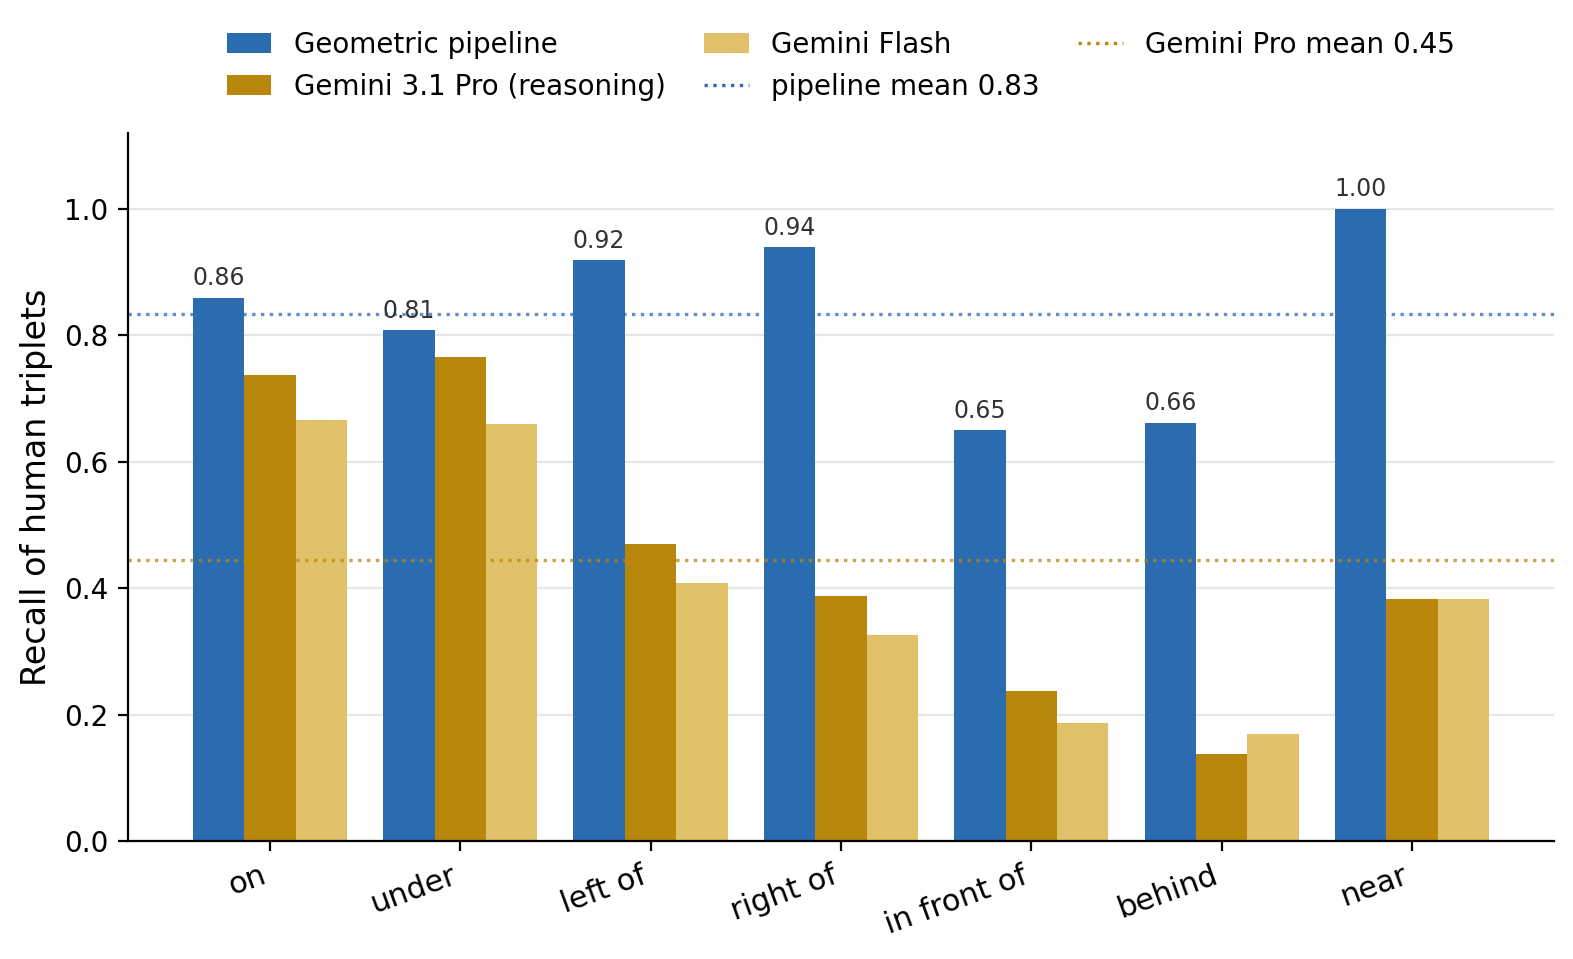
\includegraphics[width=0.80\textwidth,height=0.78\textheight,keepaspectratio]{figures/rq1-with-vlm.png}
\caption[Recall of the human triplets per predicate: the geometric]{Recall of the human triplets per predicate: the geometric pipeline against both vision-language models on the same 30 images, the same numbered boxes and the same written definitions. The dotted lines are the two means. Scaling the model lifts every predicate a little and closes none of the gap.}
\label{fig:rq1-with-vlm}
\end{figure}


All three baselines of \S{}4.2 are deliberately weak. The strong one is a vision-language model, and if it annotates this dataset as well as the geometric pipeline does, the pipeline is unnecessary. I ran two of them on thirty images under Chapter 3's own definitions, in the same PredCls setting, one small and non-reasoning and one a reasoning model an order of magnitude larger. Figure~\ref{fig:rq1-with-vlm} plots both against the pipeline, and the setting, the per-predicate tables, the diagnostics and the limits of a thirty-image pilot are in Supplementary E.1.

Both lose on recall everywhere, 0.400 and 0.445 against the pipeline's 0.834, so neither model closed the gap in this pilot, on thirty images. But recall rewards whoever asserts more. Restricted to the pairs both judged, \textbf{both models are more precise than the pipeline}, 0.419 and 0.389 against 0.347, while losing F1 on every predicate. Most of the recall gap is silence, because the model never addressed \textbf{171 of the 381 gold triplets}, 44.9\%, and on the pairs it did judge its recall is 0.686 rather than 0.378. What it is bad at is \textit{exhaustiveness}, which is the property this project exists to supply. So the fair statement is that the pipeline beats it on coverage and matches it on judgement. What decides the reading is the shape of the failure. Neither model contradicts itself or inverts the convention. They fall silent, and they supply one direction of a symmetric pair without the other in a third of cases. Those are the two defects \S{}4.5 measures in the \textit{human} annotation. Asked to annotate, a capable vision-language model reproduces the characteristic failure of the human process, not a geometric one. Its precision where it does speak still begins a case for using it as an adjudicator on the depth pair (\S{}7.6).

\section{Auditing the audit: blinding, decoys, and a second judge}

Every precision figure so far rests on the author verdicting the author's own tool, which is the objection \S{}2.9 raises and \S{}7.4 concedes. More verdicts of the same kind would only narrow an interval around a possibly biased centre. So this section re-runs the audit with the three defects of \S{}4.4 and \S{}4.9 removed at once.

\textbf{Design.} 242 items: 214 claims the tool emitted and \textbf{28 decoys}, relations it did \textit{not} emit and no annotator labelled, mixed in unmarked. What makes it an instrument is the decoys. An auditor who simply agreed with every item would have scored 100\% on the earlier sheets and scores zero here. Those same 242 images went to \texttt{gemini-3.6-flash} as a second judge, independent of me. That name is the concrete snapshot the \texttt{gemini-flash-latest} alias resolved to for this call, captured per item instead of assumed, because the alias moved during the project (Supplementary B). The model rejected 24 of 28 decoys against the author's 19 of 28, making it the stricter of the two, and the pair reach Cohen's $\kappa$ 0.601 over all items and 0.425 over the claims alone. That is moderate agreement, not an echo. Supplementary E.6 carries the sampling, the class guard, the key handling, the pack's per-predicate table, the argument for letting a model judge what \S{}4.13 shows it cannot annotate, and what the decoys measure about each judge.

\textbf{Both precision measurements point in opposite directions, and which way is diagnostic.} For five predicates \S{}4.3's restricted precision badly understates this audit's. For support it inverts, 0.95 and 0.93 on annotated pairs against 0.372 and 0.431 off them. Supplementary E.6 reads what that says about the human record.

Lateral, depth and proximity claims all survive, and support does not. At 0.404 it is less than half what \S{}4.9 reported, and outside any interval I had stated, with the judges disagreeing on its level, 0.404 against 0.638, while agreeing emphatically on its direction, both far below 0.9 (raw agreement 0.814, $\kappa$ 0.576). Most of the drop comes from the blinding, not from the sample, since the same rules on the same data scored 0.77 unblinded (\S{}4.9) and 0.404 blind, which is a prior the decoys remove. \textbf{\texttt{near} is the least supported number in the audit and carries the most labels}: the judges diverge on it by \textbf{0.375}, 1.000 against 0.625 on the same 24 images, under a predicate the tool emits on 43,388 ordered pairs against 717 in the human record. What caused it was a threshold fitted in a place where its error was invisible. The shipped \texttt{on\_\allowbreak{}contact\_\allowbreak{}min} 0.60 came from Supplementary D.2's fit on train F1 against gold covering \textasciitilde{}10\% of ordered pairs, so a false positive outside the gold cost the fit nothing. I fitted the repair on annotator groups 0--5, shipped at 0.85, and re-audited from scratch on a second pack of \textbf{191 claims} drawn from the new emissions. Supplementary E.6 gives that pack's construction, the sequence, and the held-out projection it declines to quote. Below, \textbf{v3} is the pre-refit pack at 0.60 and \textbf{v4} the fresh one at the shipped 0.85.

\needspace{14.8\baselineskip}
\begin{center}
\setlength{\tabcolsep}{3pt}
\footnotesize
\begin{longtable}{lrll}
\caption[Per-predicate precision of the shipped tool]{Per-predicate precision of the shipped tool: the re-fitted threshold audited on a fresh draw, beside the superseded v3 column, so the comparison is between two independent draws and not between two readings of one.}\\
\hline
Predicate & v3 author & v4 author (shipped) & v4 model \\
\hline
\endfirsthead
\hline
Predicate & v3 author & v4 author (shipped) & v4 model \\
\hline
\endhead
on & 0.372 & \textbf{14/31 0.452 [0.29, 0.62]} & 24/31 0.774 [0.60, 0.89] \\
under & 0.431 & \textbf{24/40 0.600 [0.45, 0.74]} & 35/40 0.875 [0.74, 0.95] \\
to the left of & 0.917 & \textbf{23/24 0.958 [0.80, 0.99]} & 24/24 1.000 [0.86, 1.00] \\
to the right of & 0.958 & \textbf{24/24 1.000 [0.86, 1.00]} & 24/24 1.000 [0.86, 1.00] \\
in front of & 0.958 & \textbf{21/24 0.875 [0.69, 0.96]} & 23/24 0.958 [0.80, 0.99] \\
behind & 0.917 & \textbf{23/24 0.958 [0.80, 0.99]} & 22/24 0.917 [0.74, 0.98] \\
near & 1.000 & \textbf{19/24 0.792 [0.60, 0.91]} & 16/24 0.667 [0.47, 0.82] \\
\textbf{support pooled} & 0.404 & \textbf{38/71 0.535 [0.42, 0.65]} & 59/71 0.831 [0.73, 0.90] \\
decoys rejected & 19/28 0.679 & \textbf{27/28 0.964 [0.82, 0.99]} & 26/28 0.929 [0.77, 0.98] \\
\hline
\end{longtable}
\end{center}

Shown in the middle column is the shipped tool, and the 0.79--1.00 range quoted elsewhere for the non-support predicates is \texttt{near} at its floor and \texttt{to the right of} at its ceiling. The change is confirmed, though the projection was optimistic, since both judges record a large improvement on an independent draw, and both record it below the 0.667 the held-out fit predicted, with held-out support recall falling from 0.92 to 0.843 in exchange. Supplementary E.6 reads what fitting on one audit and validating on the next can and cannot establish, and why neither the auditor's own improvement between the packs nor the model's parallel movement rescues the support figure. At 0.535, the labels the tool adds beyond the human record on this predicate are right about half the time.

\section{Summary}

Measured against the 8,926 relationships the annotators recorded, and \S{}4.8 gives the answer per predicate and per axis. Precision on the labels the tool adds beyond that record went through two instruments of increasing severity, an author audit and then a blind decoy-controlled re-audit with a second judge, which agree on where it holds and where it does not. Every remaining disagreement is attributed to a cause, leaving about 7\% of the misses as avoidable tool error, and two checks needing no gold at all bound what the gold itself can settle. Chapter 5 turns from whether the labels are accurate to whether they are useful, training the same relation model once on each label source.